\documentclass[a4paper,ngermanб,12pt]{article}


%%%%%%%%%%%%%%%%%%%%%%%%%%%%%%%%%%%%%%%%%%%%%%%%%%%%%%%%%%%%%%%%%%%%%%%%%%%%%%%%%%%%%%%%%%%%%%%%%%%
%% allgemeine LaTeX Pakete laden
%%%%%%%%%%%%%%%%%%%%%%%%%%%%%%%%%%%%%%%%%%%%%%%%%%%%%%%%%%%%%%%%%%%%%%%%%%%%%%%%%%%%%%%%%%%%%%%%%%%

% Mathematik
\usepackage{amsmath}  % American Math Society Packete: general
\usepackage{amsfonts} % American Math Society Packete: more fonts
\usepackage{amssymb}  % American Math Society Packete: more symbols
\usepackage{stmaryrd} % St Mary Road symbols for theoretical computer science
\usepackage[framed,hyperref,amsmath,thmmarks]{ntheorem} % en­hance­ments for the­o­rem-like en­vi­ron­ments

% Umlaute tippen
\usepackage[utf8]{inputenc}

% Wörterbuch für korrekte Silbentrennung, Titel von Abschnitten (Abbildung, Zusammenfassung, Literaturverzeichnis)
\usepackage{babel}

% Blockweises auskommentieren mit \begin{comment}\end{comment}
\usepackage{verbatim}

% Grafiken 
\usepackage{graphics,graphicx} % Bilder
\usepackage{color,xcolor} % Farbnamen
\graphicspath{{figures/}} % Es gibt ein Unterverzeichnis, wo alle Bilder liegen. Durch diesen Befehl muss man nicht jedes mal den Dateipfad angeben

%Listen
\usepackage{enumerate}
\usepackage{enumitem}

%Tabellen
\usepackage{tabularx}
\usepackage{booktabs}% Statt \hline kann \toprule, \midrule und \bottomrule verwendet werden.
\usepackage{longtable}
\usepackage{tabularray}
\usepackage{multicol} % to use columns with multiple rows
%\usepackage{multirow} % provides a construction for table cells that span more than one row

% Algorithmen
\usepackage{algorithm}
\usepackage{algorithmic}
% Algorithmen auf Deutsch %
\renewcommand{\algorithmicrequire}{\textit{Eingabe:}}
\renewcommand{\algorithmicensure}{\textit{Ausgabe:}}
\floatname{algorithm}{Algorithmus}

%Referenzen
\usepackage[unicode,pdfmenubar,linktoc=all,hidelinks,bookmarks]{hyperref} % ermöglicht PDF-Verklinkungen
\usepackage{url} % al­lows line­breaks at cer­tain char­ac­ters in urls/ e-mail adresses/ paths
%\usepackage{thmtools}%für nameref von Theoremen, aber dann sind Nummern bei Lemma/Korollar weg
\usepackage[nameinlink, compress, sort]{cleveref}% Kommando \Cref{label} schreit automatisch Abbildung/Abschnitt/Tabelle vor die Referenz
\usepackage{nameref}

%%%%%%%%%%%%%%%%%%%%%%%%%%%%%%%%%%%%%%%%%%%%%%%%%%%%%%%%%%%%%%%%%%%%%%%%%%%%%%%%%%%%%%%%%%%%%%%%%%%
%% Tikz Grafiken
%%%%%%%%%%%%%%%%%%%%%%%%%%%%%%%%%%%%%%%%%%%%%%%%%%%%%%%%%%%%%%%%%%%%%%%%%%%%%%%%%%%%%%%%%%%%%%%%%%%
\usepackage{tikz}
% Zusätzliche Tikz-Module einbinden
\usetikzlibrary{automata} 
\usetikzlibrary{arrows}
\usetikzlibrary{calc}
\usetikzlibrary{positioning}

% Tikz-Stil für Automaten
\tikzset{
	myautomat/.style = {
		>=stealth, shorten >= 1pt,auto,node distance=2cm,
	}
}
\tikzstyle{initial}+=[initial text=]

%Definiere hier eigene Tikz-Styles, damit alle Grafiken (z.B. alle Graphen) in einem einheitlichen Stil sind

%%%%%%%%%%%%%%%%%%%%%%%%%%%%%%%%%%%%%%%%%%%%%%%%%%%%%%%%%%%%%%%%%%%%%%%%%%%%%%%%%%%%%%%%%%%%%%%%%%%
%% Literatur
%%%%%%%%%%%%%%%%%%%%%%%%%%%%%%%%%%%%%%%%%%%%%%%%%%%%%%%%%%%%%%%%%%%%%%%%%%%%%%%%%%%%%%%%%%%%%%%%%%%
\usepackage[style=alphabetic,backend=biber]{biblatex}
\bibliography{literatur}

%%%%%%%%%%%%%%%%%%%%%%%%%%%%%%%%%%%%%%%%%%%%%%%%%%%%%%%%%%%%%%%%%%%%%%%%%%%%%%%%%%%%%%%%%%%%%%%%%%%
%% Theoreme 
%%%%%%%%%%%%%%%%%%%%%%%%%%%%%%%%%%%%%%%%%%%%%%%%%%%%%%%%%%%%%%%%%%%%%%%%%%%%%%%%%%%%%%%%%%%%%%%%%%%

%Definiere Umgebungen für Aussagen
\newtheorem{theorem}{Theorem}% (wichtiger Satz) Höhepunkt in der Entwicklung einer Theorie
\newtheorem{corollary}[theorem]{Korollar}% (Folgerung) einfach/ trivial aus vorhergehenden Sätzen zu folgern 
\newtheorem{lemma}[theorem]{Lemma}% (Hilfssatz) rein technische Aussage, als Schlüsselgedanke für anderen Beweis
\newtheorem{proposition}[theorem]{Proposition}%  Mittelding aus Hilfssatz und Theorem
\newtheorem{observation}[theorem]{Beobachtung}

\newtheorem{example}[theorem]{Beispiel}
\newtheorem{definition}[theorem]{Definition}
\newtheorem{problem}[theorem]{Problem}
\newtheorem{remark}[theorem]{Bemerkung}

% Beweis-Umgebung
\theorembodyfont{\upshape}
\theoremstyle{nonumberplain}
\theoremheaderfont{\itshape}
\theoremsymbol{\ensuremath{\Box}}%QED Symbol am Beweisende
\newtheorem{proof}{Beweis}

% Zeilennummern
\usepackage{lineno}

%%%%%%%%%%%    Meta Informationen   %%%%%%%%%%%%%%
\title{Min-Cost Max-Flow\\
{\normalsize Proseminar:  Fortgeschrittene Algorithmen für Programmierwettbewerbe
}
}
\author{Vladimir Vassilyev}
\date{\today}

\begin{document}

\maketitle

%%%%%%%%%%%    Ausarbeitung   %%%%%%%%%%%%%%
\linenumbers % Ab hier werden die Zeilen gezählt
	
\begin{abstract}

In meiner Ausarbeitung geht es um Min-Cost Max-Flow - ein Algorithmus, das echt hilfreich bei der Lösung verschiedenster Problemen sein kann und dabei ganz leicht zu verstehen und implementieren ist. Ich werde heute Implementierung von diesem Algorithmus zeigen und erklären. Außerdem will ich paar Beispielaufgaben, u.a. aus den echten Programmierwettbewerben vorzeigen, die mithilfe von Min-Cost Flow gelöst werden können.
\end{abstract}

\section{Einleitung}
\label{sec:intro}
Führe hier in das Thema ein: Worum geht es? Warum ist dies interessant? Welche Ergebnisse werden vorgestellt? Aufbau der Arbeit?

  Alles in unserer Welt ist irgendwie miteinander verbunden. Diese enge Verbundenheit kann mithilfe von Graph bezeichnet werden. Graph ist eine Datenstruktur, die in der Programmierung, u.a. in Programmierwettbewerben seit langem verwendet wurde. Diese Datenstruktur hilft uns, komplexe Probleme aus der echten Welt auf eine neue Ebene zu reduzieren und besseres Verständnis davon zu kriegen. In meiner Arbeit betrachte ich das Algorithmus Min-Cost (Max) Flow näher. Es ist ein guter Beispiel der Nutzung von Graphen.  \newline
 
\newpage

\section{Problemstellung}



\subsection{Definition}

 Wie kann man denn Min-Cost Max-Flow beschreiben? Im Buch "Competitive Programming 4"  wurde es so beschrieben: \newline 
  \normalsize
   The Min Cost Flow problem is the problem of finding the cheapest possible way of sending a certain amount of (not necessarily the max) flow through a flow network.\cite{Halim2018} \newline
   Kurz gesagt, man soll den effizientesten Weg mit maximalem Fluss aus dem gesamten Graph finden. Effizient bedeutet in diesem Kontext, dass die Flusswege auch ihre Kosten haben können. Damit es bisschen verständlicher wird, gebe ich eine typische Aufgabe zu diesem Algorithmus.

\subsection{Beispiel}
Hier ist ein Beispiel der Aufgabe, der mithilfe von Min-Cost Max-Flow gelöst wird:

\begin{figure}[H]
    \centering
    \includegraphics[width=8cm]{figures/beispiel1.png}
    \caption{Fluss-Graph \cite{Halim2018, Figure 9.23}}
\end{figure}
Wir haben hier einen Graph, wobei jede Kante ihre Kosten hat, die oben geschrieben sind. Jeder Pfad hat eine Flusskapazität von 10 Einheiten. In dieser Aufgabe wollen wir 20 Einheiten von Fluss von A nach D übertragen. Wir sollen den effizientesten Weg dazu finden. Es gibt insgesamt drei mögliche Lösungen:
\begin{itemize}
    \item A$\rightarrow$D + A$\rightarrow$B$\rightarrow$D = 1*10 + (3+4)*10 = 80 
    \item A$\rightarrow$D + A$\rightarrow$C$\rightarrow$D = 1*10 + (3+5)*10 = 90 
    \item A$\rightarrow$C$\rightarrow$D + A$\rightarrow$B$\rightarrow$D = (3+4)*10 + (3+5)*10 = 150 
\end{itemize}
Wie wir sehen können braucht die erste Variante am wenigsten Kosten, deswegen wählen wir die aus. Aber was wenn wir eine komplexere Aufgabe haben? Wie genau funktioniert das Algorithmus? Das erkläre ich im nächsten Kapitel.

\newpage

\section{Implementierung}

\subsection{Auswahl des Algorithmus}
Jetzt betrachten wir, wie Min-Cost Flow Algorithmus am besten implementiert werden kann. Bevor wir mit der Implementierung beginnen, sollen wir einen Aspekt betrachten: die Kosten können auch negativ sein, da wir die Kosten dieses augmentierenden Pfades subtrahieren müssen, da das Aufheben des Flusses bedeutet, dass wir diese Kante nicht verwenden wollen.\cite{Halim2018} \newline Warum ist das wichtig? In manchen Situationen können negative Zyklen entstehen. Ein negativer Zyklus im Kosten-Netzwerk entsteht, wenn die Summe der Kosten aller Kanten im Zyklus negativ ist. Diese können mit dem \textbf{Bellman-Ford-Algorithmus} erkannt werden. Sie sollten beseitigt werden, da der Fluss durch solche Zyklen in der Praxis nicht zulässig ist. Betrachten wir einen negativen Kostenzyklus: Wenn der gesamte Fluss diesen Zyklus durchlaufen muss, verringern sich die Gesamtkosten mit jedem abgeschlossenen Zyklus. Dies würde zu einer Endlosschleife führen, wenn man die Gesamtkosten minimieren möchte. Wenn ein Kosten-Netzwerk also einen negativen Zyklus enthält, bedeutet dies, dass die Kosten weiter minimiert werden können\cite{GeeksforGeeks2023}(übersetzt durch DeepL).

\subsection{Schrittweise Aufteilung}
Ian Kiprono, Senior Software Developer bei PInterest, hat einen Artikel zu diesem Thema auf der Webseite geeksforgeeks.com hochgeladen. Lasst uns, mithilfe von obengenanntem Artikel\cite{GeeksforGeeks2023}, zuerst das Algorithmus schrittweise aufteilen (übersetzt durch DeepL):
\begin{enumerate}
    \item Speichern Sie die Kapazität einer Kante und die Kosten dieser Kante in zwei separaten Arrays.
    \item Gegeben seien der Quellknoten $\mathbf{S}$ und der Senkenknoten $\mathbf{T}$, die ausgewählte Kante $\mathbf{p_i}$, die Nachfragknoten $\mathbf{d_a}$ und die Entfernung zwischen den Knoten $\mathbf{dist}$. Suchen Sie, ob es möglich ist, einen Fluss von $\mathbf{S}$ nach $\mathbf{T}$ zu haben.
    \item Wenn ein Fluss existiert, berechnen Sie die Entfernung, Wert = $\mathbf{dist}$ + $\mathbf{p_i}$ – $\mathbf{p_i}$[k] - $\mathbf{cost}$[k].
    \item Vergleichen Sie die Entfernungswerte in $\mathbf{dist}$[ ] mit dem Wert und aktualisieren Sie so lange, bis der minimale Fluss erreicht ist.
\end{enumerate}
Wir können also drei wichtigste Unterprobleme definieren\cite{Cruz2023}:
\begin{itemize}
    \item Shortest $(s,t)$-path Problem – Wir haben einen Digraphen $G$, zwei bestimmte Knoten $\mathbf{s}$ und $\mathbf{t}$ und einen Kostenvektor $c \in \mathbb{Q}^m$. Die Aufgabe besteht darin, einen Pfad von $\mathbf{s}$ nach $\mathbf{t}$ mit minimalen Gesamtkosten zu finden.
    
    \item Transshipment problem –  die Variante von MCF, bei der keine Kantenkapazitäten vorhanden sind (oder, gleichbedeutend, alle Kantenkapazitäten sehr groß sind) 
    
    \item Negative-cycle detection problem –  Wir haben einen Digraphen $G$ und einen Kostenvektor $c \in \mathbb{Z}^m$. Die Aufgabe besteht darin, zu überprüfen, ob
 es in $G$ einen gerichteten Zyklus gibt, dessen Gesamtkosten negativ sind. (übersetzt durch DeepL)
\end{itemize}
Wir haben die Unterprobleme nicht nur für besseres Verständnis des Algorithmus erwähnt. Die können auch für genauere Analyse der Laufzeit, die wir später durchführen, hilfreich sein. 
\subsection{Code}
Hier ist ein Pseudo-Code für das Algorithmus, das Min-Cost Max-Flow Problem löst\cite{GeeksforGeeks2023}:
\begin{algorithm}
	\caption{Wieviel Fluss kann gesendet werden?}
	\label{alg:BFS}
	\begin{algorithmic} []
		\REQUIRE Kapazitätenarray $cap$, Flussarray $flow$, Quellknoten $src$, Senkenknoten $sink$
		%\ENSURE BFS
		
		%\STATE	$Q$.enqueue($s$)			
		%\STATE mark $s$ as visited
		%\WHILE{$Q$ is not empty}
		%\STATE	$v$ = $Q$.dequeue( )			
		%\FORALL{neighbors $w$ of $v$}
		%\IF{$w$ is not visited}
		%\STATE	$Q$.enqueue($w$)
		%\STATE	mark $w$ as visited
		%\ENDIF
		%\ENDFOR
		%\ENDWHILE
        \STATE $amt \gets INF$
        \STATE $x \gets sink$
        \IF{$flow[x][dad[x]] \neq 0$}
        \STATE $val \gets flow[x][dad[x]]$
        \ELSE
        \STATE $val \gets cap[dad[x]][x] - flow[dad[x]][x]$
        \ENDIF

    
        \WHILE{$x$ != $src$}
        \STATE $amt \gets \min( amt, val  )$

        \ENDWHILE
	\end{algorithmic}
\end{algorithm}
\newpage
\section{Laufzeit und Korrektheit}


Gebe hier eine abgeschlossene Darstellung des Inhaltes. Schreibe diese so, dass sie für Deine Kommilitonen verständlich ist. Verwende dabei zur Anschauung des Inhaltes auch Beispiele und Abbildungen.

\subsection{Hinweise}

Der Hauptteil soll natürlich nicht den Titel \glqq Hauptteil\grqq\ sondern einen passenden Titel haben, und zudem in sinnvolle Abschnitte und Unterabschnitte mit passenden Überschriften gegliedert sein.\\

\subsection{Zitate und Referenzen}
Denke daran, alle Aussagen durch Quellen zu belegen. Beispielsweise die Aussage, dass Turing die Unentscheidbarkeit des Halteproblems gezeigt hat \cite{Turing1937}.
\newpage
\section{Maximum Flow}


Gebe hier eine abgeschlossene Darstellung des Inhaltes. Schreibe diese so, dass sie für Deine Kommilitonen verständlich ist. Verwende dabei zur Anschauung des Inhaltes auch Beispiele und Abbildungen.

\subsection{Hinweise}

Der Hauptteil soll natürlich nicht den Titel \glqq Hauptteil\grqq\ sondern einen passenden Titel haben, und zudem in sinnvolle Abschnitte und Unterabschnitte mit passenden Überschriften gegliedert sein.\\

\subsection{Zitate und Referenzen}
Denke daran, alle Aussagen durch Quellen zu belegen. Beispielsweise die Aussage, dass Turing die Unentscheidbarkeit des Halteproblems gezeigt hat \cite{Turing1937}.
\newpage

\section{Beispiele}


Gebe hier eine abgeschlossene Darstellung des Inhaltes. Schreibe diese so, dass sie für Deine Kommilitonen verständlich ist. Verwende dabei zur Anschauung des Inhaltes auch Beispiele und Abbildungen.

\subsection{Hinweise}

Der Hauptteil soll natürlich nicht den Titel \glqq Hauptteil\grqq\ sondern einen passenden Titel haben, und zudem in sinnvolle Abschnitte und Unterabschnitte mit passenden Überschriften gegliedert sein.\\

\subsection{Zitate und Referenzen}
Denke daran, alle Aussagen durch Quellen zu belegen. Beispielsweise die Aussage, dass Turing die Unentscheidbarkeit des Halteproblems gezeigt hat \cite{Turing1937}.



Um innerhalb der Ausarbeitung zu referenzieren, können Bereiche mit einem \texttt{label} versehen werden. Durch das Paket \texttt{cleverref} wird beim Referenzieren automatisch [Abbildung/ Abschnitt/ Tabelle/ etc.] ergänzt. Beispiele in diesem Dokument sind \Cref{sec:intro,fig:automat,alg:BFS,theo:aussage}.

\begin{figure}
	\centering
	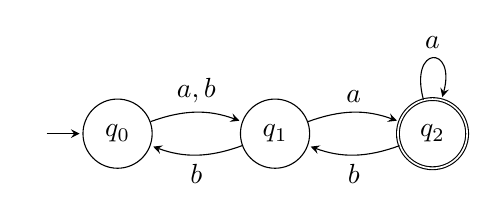
\begin{tikzpicture}[myautomat]
		\node[state, initial] (0) {$q_0$};
		\node[state] (1) [right of=0] {$q_1$};
		\node[state, double] (2) [right of=1] {$q_2$};
		
		\draw[->] (0) edge[bend left=20] node[auto] {$a,b$} (1);
		\draw[->] (1) edge[bend left=20] node[auto] {$a$} (2)
		edge[bend left=20] node[auto] {$b$} (0);
		\draw[->] (2) edge[loop above] node[auto] {$a$} () 
		edge[bend left=20] node[auto] {$b$} (1);
	\end{tikzpicture}
	\caption{Ein Automat, der mit Tikz erzeugt wurde}
	\label{fig:automat}
\end{figure}

\begin{figure}
	\centering
	\includegraphics[width=8cm]{automat.jpg} 
	\caption{Eine Automat, der als jpg-Bild eingebunden wurde (Achtung: Auflösung!)}
\end{figure}

\begin{theorem}[Besondere Formel]\label{theo:aussage}
	Hier ist eine Aussage.
\end{theorem}
\begin{proof}
	Hier folgt der Beweis.
\end{proof}




\section{Zusammenfassung und Ausblick}

Fasse hier die vorgestellten Ergebnisse zusammen, diskutiere diese und gebe einen Ausblick auf offene Fragen. 

%%%%%%%%%%%    Der folgende Teil zählt nicht zu Zeilenbeschränkung der Vorgabe   %%%%%%%%%%%%%%
\nolinenumbers

%%%%%%%%%%%    Literaturverzeichnis   %%%%%%%%%%%%%%
 \printbibliography 
 
 %%%%%%%%%%%    Anhang   %%%%%%%%%%%%%%
 \appendix
 
 \section{Eigenständigkeitserklärung und verwendete Hilfsmittel}
Ich versichere an Eides statt, dass ich die vorliegende Arbeit in allen Teilen selbstständig und ohne unzulässige Hilfe Dritter absolviert sowie keine anderen als die genannten und explizit zugelassenen Hilfsmittel verwendet und mich im Allgemeinen prüfungskonform verhalten habe. Ich erkläre zudem, dass ich beim Einsatz von IT-/KI-gestützten Schreibwerkzeugen diese Werkzeuge in der Übersicht verwendeter Hilfsmittel mit ihrem Produktnamen, meiner Bezugsquelle und … vollständig aufgeführt und/oder die betreffenden Textstellen in der Arbeit als mit KI generierter Unterstützung verfasst gekennzeichnet habe. Mir ist bewusst, dass Täuschungen bzw. Täuschungsversuche nach der für mich geltenden Prüfungsordnung geahndet werden.\\


Folgende Hilfsmittel habe ich für die Bearbeitung genutzt:
DeepL Übersetzer
 
\end{document}